\documentclass[a4paper,12pt]{article}

\usepackage[T2A]{fontenc}
\usepackage[utf8]{inputenc}
\usepackage[russian]{babel}

\usepackage[margin=2cm]{geometry}
\usepackage{amsmath, amssymb}

\usepackage{graphicx}
\graphicspath{{assets}}

\usepackage{array}
\usepackage{float}
\usepackage{longtable}
\usepackage{multirow}
\usepackage{setspace}

\usepackage{hyperref}
\hypersetup{%
    colorlinks=true,
    linkcolor=blue,
    filecolor=magenta,
    urlcolor=magenta,
}

\setlength{\parindent}{0pt}

\newcommand\Section[1]{%
\refstepcounter{section}%
\section*{%
\raggedright
\arabic{section}. #1
}%
\addcontentsline{toc}{section}{\arabic{section}. #1}%
}

\newcommand\Subsection[1]{%
\refstepcounter{subsection}%
\subsection*{%
\raggedright%
\arabic{section}. \arabic{subsection}. #1
}%
\addcontentsline{toc}{subsection}{\arabic{subsection}. #1}%
}

\begin{document}

% ---------- HEADER ----------

\begin{minipage}{0.55\textwidth}
    \begin{center}
        \textbf{Университет ИТМО}\\
        Физико-технический факультет\\
        Физический факультет
    \end{center}
\end{minipage}
\hfill
\begin{minipage}{0.35\textwidth}
    \begin{flushright}
        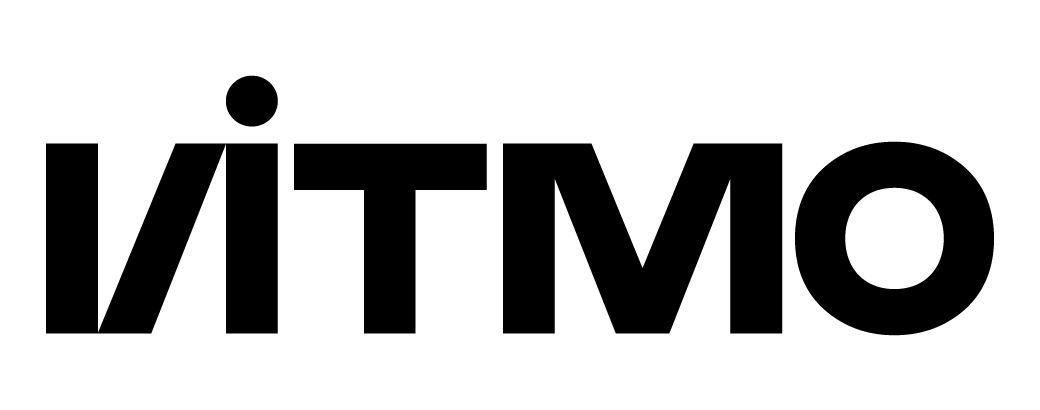
\includegraphics[width=3.2cm]{assets/itmo_logo.png}
    \end{flushright}
\end{minipage}

\vspace{1.2cm}

\begin{tabular}{@{}p{7cm}p{6cm}@{}}
Группа\hspace{0.3cm}%
\makebox[4cm]{\rlap{\raisebox{0.3ex}{\hspace{1.0cm}ПИИКТ 2.2}}\hrulefill}
&
К работе допущен \hrulefill
\\[0.8cm]
Студент\hspace{0.3cm}%
\makebox[4cm]{\rlap{\raisebox{0.3ex}{\hspace{0.5cm}Бых Д. М.}}\hrulefill}
&
Работа выполнена \hrulefill
\\[0.8cm]
Преподаватель\hspace{0.2cm}%
\makebox[3cm]{\rlap{\raisebox{0.3ex}{\hspace{0.5cm}Рудель А. Е.}}\hrulefill}
&
Отчет принят \hrulefill
\end{tabular}

\vspace{1.2cm}

\begin{center}
{\Large\bfseries Рабочий протокол и отчет по\\ лабораторной работе №1.04}
\vspace{1cm}

{\large \textit{Исследование равноускоренного вращательного движения (маятник Обербека)}}
\end{center}

\vspace{2cm}

\Section{Цель работы}
\begin{enumerate}
    \item Определение массы вращающегося тела.
    \item Проверка зависимости момента инерции системы от распределения масс в системе.
\end{enumerate}

\Section{Задачи, решаемые при выполнении работы}
\begin{enumerate}
    \item Экспериментально исследовать зависимость углового ускорения от момента раскручивающей силы для тела, вращающегося вокруг неподвижной оси.
    \item Из графика экспериментальной зависимости момента раскручивающей силы от углового ускорения вычислить момент инерции тела и момент силы трения.
    \item Из графика экспериментальной зависимости момента инерции системы тел от их расстояния до оси вращения вычислить массу тела.
    \item Исследовать зависимость момента инерции системы тел от их расстояния до оси вращения.
\end{enumerate}

\Section{Объект исследования}
Маятник Обербека (крестовина со ступенчатой ступицей и четырьмя спицами с перемещаемыми грузами).

\Section{Метод экспериментального исследования}
Экспериментальное наблюдение равноускоренного поступательного опускания каретки с шайбами и связанного с ним вращения крестовины. Обработка данных методом наименьших квадратов (МНК).

\Section{Рабочие формулы и исходные данные}

Линейное ускорение каретки:
\[
a = \frac{2h}{t^2}.
\]
Связь линейного и углового ускорений:
\[
\varepsilon = \frac{2a}{d},
\]
где $d$ — диаметр ступицы.
Момент силы натяжения нити:
\[
M = \frac{md}{2}(g - a),
\]
где $m$ — масса каретки с шайбами.

Основной закон динамики вращательного движения с учётом момента силы трения $M_{\text{тр}}$:
\[
M = I\varepsilon + M_{\text{тр}}.
\]

Теорема Штейнера:
\[
I = I_0 + 4m_{\text{гр}}R^2.
\]

Расстояние от оси до центра масс груза на крестовине:
\[
R = \ell_1 + (n-1)\ell_0 + \frac{b}{2}.
\]

\noindent\textbf{Исходные данные (паспортные параметры стенда):}\\
\(h = (0.700 \pm 0.001)\) м, \(g = (9.81 \pm 0.01)\) м/с\(^2\);\\
\(m_{\text{к}} = (0.0480 \pm 0.0005)\) кг, \(m_{\text{ш}} = (0.2180 \pm 0.0005)\) кг;\\
\(d = (0.0460 \pm 0.0005)\) м, \(b = (0.0400 \pm 0.0005)\) м;\\
\(\ell_1 = (0.0570 \pm 0.0005)\) м, \(\ell_0 = (0.0250 \pm 0.0002)\) м;\\
\(m_{\text{гр}}^{\text{пасп}} = (0.4050 \pm 0.0005)\) кг;\\
масса каретки с $N$ шайбами: \(m = m_{\text{к}} + N m_{\text{ш}}\);\\
погрешность массы: \(\Delta m = \sqrt{\Delta m_{\text{к}}^2 + \Delta m_{\text{ш}}^2} \approx 0.0007\) кг.

\Section{Измерительные приборы}
\begin{table}[H]
    \centering
    \renewcommand{\arraystretch}{1.4}
    \begin{tabular}{|c|p{5cm}|p{3cm}|p{3cm}|}
        \hline
        \textit{№} & \textit{Наименование} & \textit{Используемый диапазон} & \textit{Погрешность} \\
        \hline
        1 & Электронный секундомер & $0 - 99.99$ с & \(\pm 0.01\) с \\
        \hline
        2 & Миллиметровая линейка & $0 - 1000$ мм & \(\pm 1\) мм \\
        \hline
    \end{tabular}
\end{table}

\Section{Схема установки}
\begin{figure}[H]
    \centering
    \fbox{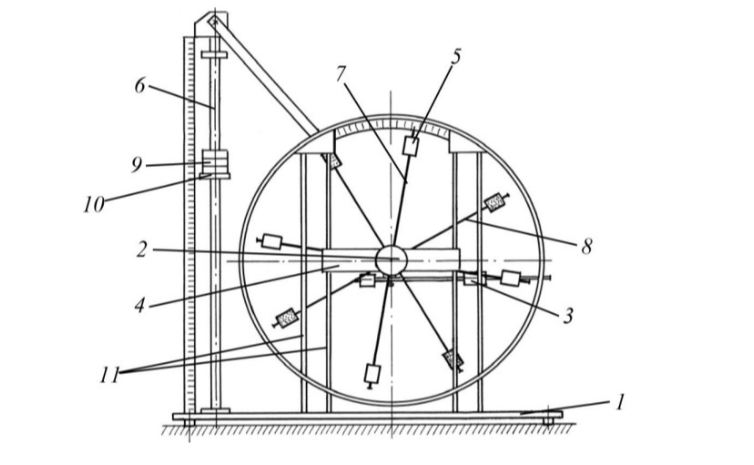
\includegraphics[width=0.75\textwidth]{assets/scheme_1_04.png}}
    \caption{Схема экспериментального стенда}
    \label{fig:scheme}
\end{figure}
В состав экспериментального стенда входят:
\begin{enumerate}
    \item Основание
    \item Рукоятка сцепления крестовин
    \item Устройства принудительного трения
    \item Поперечина
    \item Груз крестовины
    \item Трубчатая направляющая
    \item Передняя крестовина
    \item Задняя крестовина
\end{enumerate}

\Section{Результаты прямых измерений}
В Таблице~1 приведены результаты измерений времени падения каретки для четырёх положений грузов на крестовине (риски 1--4) и четырёх вариантов массы каретки (1--4 шайбы). В каждой ячейке выполнено $n = 3$ измерения.

\begin{table}[H]
    \centering
    \caption{Среднее время падения каретки с шайбами}
    \small
    \begin{tabular}{|c|c|c|c|c|c|}
        \hline
        \multirow{2}{*}{Риска} & \multirow{2}{*}{Шайб, шт} & \multicolumn{3}{c|}{Время, с} & \multirow{2}{*}{\(\langle t \rangle\), с} \\
        \cline{3-5}
        & & \(t_1\) & \(t_2\) & \(t_3\) & \\
        \hline
        \multirow{4}{*}{1} & 1 & 4.61 & 4.63 & 4.55 & 4.597 \\
        \cline{2-6}
        & 2 & 3.12 & 3.15 & 3.13 & 3.133 \\
        \cline{2-6}
        & 3 & 2.54 & 2.56 & 2.55 & 2.550 \\
        \cline{2-6}
        & 4 & 2.20 & 2.24 & 2.23 & 2.223 \\
        \hline
        \multirow{4}{*}{2} & 1 & 5.18 & 5.22 & 5.21 & 5.203 \\
        \cline{2-6}
        & 2 & 4.09 & 4.13 & 4.11 & 4.110 \\
        \cline{2-6}
        & 3 & 3.35 & 3.38 & 3.36 & 3.363 \\
        \cline{2-6}
        & 4 & 2.65 & 2.68 & 2.67 & 2.667 \\
        \hline
        \multirow{4}{*}{3} & 1 & 5.67 & 5.71 & 5.70 & 5.693 \\
        \cline{2-6}
        & 2 & 4.24 & 4.28 & 4.26 & 4.260 \\
        \cline{2-6}
        & 3 & 3.45 & 3.49 & 3.47 & 3.470 \\
        \cline{2-6}
        & 4 & 3.17 & 3.20 & 3.19 & 3.187 \\
        \hline
        \multirow{4}{*}{4} & 1 & 6.52 & 6.56 & 6.55 & 6.543 \\
        \cline{2-6}
        & 2 & 5.22 & 5.27 & 5.25 & 5.247 \\
        \cline{2-6}
        & 3 & 4.00 & 4.04 & 4.02 & 4.020 \\
        \cline{2-6}
        & 4 & 3.49 & 3.52 & 3.51 & 3.507 \\
        \hline
    \end{tabular}
\end{table}

\Section{Расчёт результатов косвенных измерений}

\Subsection{Пример расчёта для первой точки (Риска 1, 1 шайба)}
\begin{align*}
\langle t \rangle &= \frac{4.61 + 4.63 + 4.55}{3} = 4.597\ \text{с},\\
a &= \frac{2 \cdot 0.700}{(4.597)^2} = 0.0662\ \text{м/с}^2,\\
\varepsilon &= \frac{2 \cdot 0.0662}{0.0460} = 2.878\ \text{рад/с}^2,\\
M &= \frac{(0.048 + 0.218) \cdot 0.0460}{2} (9.81 - 0.0662) = 0.0596\ \text{Н}\cdot\text{м}.
\end{align*}

\Subsection{Результаты расчётов для всех серий}
\begin{table}[H]
    \centering
    \caption{Результаты косвенных измерений \(a\), \(\varepsilon\) и \(M\)}
    \small
    \begin{tabular}{|c|c|c|c|c|}
        \hline
        Риска & Шайб & \(a\), м/с\(^2\) & \(\varepsilon\), рад/с\(^2\) & \(M\), Н\(\cdot\)м \\
        \hline
        \multirow{4}{*}{1} & 1 & 0.0662 & 2.878 & 0.0596 \\
        \cline{2-5}
        & 2 & 0.1425 & 6.196 & 0.1076 \\
        \cline{2-5}
        & 3 & 0.2149 & 9.343 & 0.1549 \\
        \cline{2-5}
        & 4 & 0.2835 & 12.326 & 0.2016 \\
        \hline
        \multirow{4}{*}{2} & 1 & 0.0517 & 2.248 & 0.0597 \\
        \cline{2-5}
        & 2 & 0.0829 & 3.604 & 0.1083 \\
        \cline{2-5}
        & 3 & 0.1237 & 5.378 & 0.1564 \\
        \cline{2-5}
        & 4 & 0.1971 & 8.570 & 0.2034 \\
        \hline
        \multirow{4}{*}{3} & 1 & 0.0432 & 1.878 & 0.0597 \\
        \cline{2-5}
        & 2 & 0.0771 & 3.352 & 0.1083 \\
        \cline{2-5}
        & 3 & 0.1163 & 5.057 & 0.1565 \\
        \cline{2-5}
        & 4 & 0.1381 & 6.004 & 0.2047 \\
        \hline
        \multirow{4}{*}{4} & 1 & 0.0327 & 1.422 & 0.0598 \\
        \cline{2-5}
        & 2 & 0.0509 & 2.213 & 0.1086 \\
        \cline{2-5}
        & 3 & 0.0866 & 3.765 & 0.1570 \\
        \cline{2-5}
        & 4 & 0.1138 & 4.948 & 0.2052 \\
        \hline
    \end{tabular}
\end{table}

\Subsection{Расчёт момента инерции и момента силы трения}
По формулам МНК для зависимости \(M(\varepsilon)\) (модель \(M = I\varepsilon + M_{\text{тр}}\)) получены следующие значения:
\begin{itemize}
    \item Риска 1: \(I_1 = 0.0150\) кг\(\cdot\)м\(^2\), \(M_{\text{тр},1} = 0.0155\) Н\(\cdot\)м;
    \item Риска 2: \(I_2 = 0.0222\) кг\(\cdot\)м\(^2\), \(M_{\text{тр},2} = 0.0223\) Н\(\cdot\)м;
    \item Риска 3: \(I_3 = 0.0339\) кг\(\cdot\)м\(^2\), \(M_{\text{тр},3} = -0.0060\) Н\(\cdot\)м;
    \item Риска 4: \(I_4 = 0.0393\) кг\(\cdot\)м\(^2\), \(M_{\text{тр},4} = 0.0110\) Н\(\cdot\)м.
\end{itemize}
Средний момент трения: \(\langle M_{\text{тр}} \rangle \approx 0.011\) Н\(\cdot\)м.

\Subsection{Расчёт расстояний \(R\) и \(R^2\)}
\[
\begin{aligned}
R_1 &= 0.057 + 0 + 0.020 = 0.077\ \text{м} \implies R_1^2 = 0.00593\ \text{м}^2,\\
R_2 &= 0.057 + 0.025 + 0.020 = 0.102\ \text{м} \implies R_2^2 = 0.01040\ \text{м}^2,\\
R_3 &= 0.057 + 0.050 + 0.020 = 0.127\ \text{м} \implies R_3^2 = 0.01613\ \text{м}^2,\\
R_4 &= 0.057 + 0.075 + 0.020 = 0.152\ \text{м} \implies R_4^2 = 0.02310\ \text{м}^2.
\end{aligned}
\]

\begin{table}[H]
    \centering
    \caption{Результаты косвенных измерений \(I\), \(M_{\text{тр}}\), \(R\) и \(R^2\)}
    \begin{tabular}{|c|c|c|c|c|}
        \hline
        Риска & \(I\), кг\(\cdot\)м\(^2\) & \(M_{\text{тр}}\), Н\(\cdot\)м & \(R\), м & \(R^2\), м\(^2\) \\
        \hline
        1 & 0.0150 & 0.0155 & 0.077 & 0.00593 \\
        \hline
        2 & 0.0222 & 0.0223 & 0.102 & 0.01040 \\
        \hline
        3 & 0.0339 & $-0.0060$ & 0.127 & 0.01613 \\
        \hline
        4 & 0.0393 & 0.0110 & 0.152 & 0.02310 \\
        \hline
    \end{tabular}
\end{table}

\Subsection{Определение \(I_0\) и \(m_{\text{гр}}\) по МНК}
Согласно теореме Штейнера, \(I = I_0 + 4m_{\text{гр}}R^2\). По формулам МНК для точек \((R^2_i; I_i)\):
\[
b = \frac{\sum(R_i^2 - \overline{R^2})(I_i - \bar I)}{\sum(R_i^2 - \overline{R^2})^2} = 1.46\ \text{кг}, \qquad
I_0 = \bar I - b\overline{R^2} = 0.0073\ \text{кг}\cdot\text{м}^2.
\]
Экспериментальная масса одного груза крестовины:
\[
m_{\text{гр}}^{\text{эксп}} = \frac{b}{4} = \frac{1.46}{4} = 0.365 \approx 0.36\ \text{кг}.
\]

\Section{Расчёт погрешностей}

\Subsection{Погрешность времени для первой точки}
\begin{align*}
S_{\langle t \rangle} &= \sqrt{\frac{(4.61-4.597)^2 + (4.63-4.597)^2 + (4.55-4.597)^2}{3(3-1)}} = 0.0240\ \text{с},\\
\Delta_{\langle t \rangle} &= 4.3 \cdot 0.0240 = 0.103\ \text{с},\\
\Delta_t &= \sqrt{0.103^2 + \left(\frac{2}{3}\cdot 0.01\right)^2} \approx 0.103\ \text{с},\\
\delta_t &= \frac{0.103}{4.597} \cdot 100\% = 2.2\%.
\end{align*}

\Subsection{Погрешности \(a\), \(\varepsilon\), \(M\) для первой точки}
\begin{align*}
\delta_a &= \sqrt{\left(\frac{0.001}{0.700}\right)^2 + (2 \cdot 0.022)^2} = 4.4\%, & \Delta a &= 0.0662 \cdot 0.044 = 0.0029\ \text{м/с}^2,\\
\delta_\varepsilon &= \sqrt{0.044^2 + \left(\frac{0.0005}{0.0460}\right)^2} = 4.5\%, & \Delta \varepsilon &= 2.878 \cdot 0.045 = 0.13\ \text{рад/с}^2,\\
\delta_M &= \sqrt{\left(\frac{0.0007}{0.266}\right)^2 + \left(\frac{0.0005}{0.046}\right)^2 + \frac{0.01^2 + 0.0029^2}{(9.81 - 0.0662)^2}} = 1.1\%, & \Delta M &= 0.0596 \cdot 0.011 = 0.0007\ \text{Н}\cdot\text{м}.
\end{align*}

\Subsection{Погрешности \(I_0\) и \(m_{\text{гр}}\)}
Для $\alpha = 0.95$ по формулам МНК (с $\text{SSE} = 1.32\cdot 10^{-5}$ (кг\(\cdot\)м\(^2\))\(^2\) и $D = 1.65\cdot 10^{-4}$ м$^4$):
\begin{align*}
S_b &= \sqrt{\frac{1}{D}\frac{\text{SSE}}{N-2}} = 0.20\ \text{кг}, \qquad \Delta b = 2S_b = 0.40\ \text{кг},\\
S_a &= \sqrt{\left(\frac{1}{N} + \frac{\overline{R^2}^2}{D}\right)\frac{\text{SSE}}{N-2}} = 0.0031\ \text{кг}\cdot\text{м}^2, \qquad \Delta I_0 = 2S_a = 0.0061\ \text{кг}\cdot\text{м}^2.
\end{align*}
Следовательно:
\[
m_{\text{гр}} = (0.36 \pm 0.10)\ \text{кг}, \qquad I_0 = (7.3 \pm 6.1) \cdot 10^{-3}\ \text{кг}\cdot\text{м}^2.
\]

\Section{Графики}
\begin{enumerate}
    \item График зависимости момента силы натяжения нити от углового ускорения \(M = f(\varepsilon)\) для всех положений грузов — см.~рис.~\ref{fig:graph1}.
    \item График зависимости момента инерции от квадрата расстояния \(I = f(R^2)\) — см.~рис.~\ref{fig:graph2}.
\end{enumerate}

\Section{Окончательные результаты}
\begin{enumerate}
    \item Время падения (точка 1): \(\langle t \rangle = (4.60 \pm 0.10)\) с, \(\delta_t = 2.2\%\).
    \item Ускорение каретки (точка 1): \(a = (0.066 \pm 0.003)\) м/с\(^2\), \(\delta_a = 4.4\%\).
    \item Угловое ускорение (точка 1): \(\varepsilon = (2.88 \pm 0.13)\) рад/с\(^2\), \(\delta_\varepsilon = 4.5\%\).
    \item Момент силы натяжения (точка 1): \(M = (0.0596 \pm 0.0007)\) Н\(\cdot\)м, \(\delta_M = 1.1\%\).
    \item Масса груза на крестовине (эксперимент): \(m_{\text{гр}} = (0.36 \pm 0.10)\) кг.
    \item Собственный момент инерции крестовины: \(I_0 = (7.3 \pm 6.1) \cdot 10^{-3}\) кг\(\cdot\)м\(^2\).
    \item Средний момент сил трения: \(\langle M_{\text{тр}} \rangle \approx 0.011\) Н\(\cdot\)м.
\end{enumerate}

\Section{Выводы и анализ результатов работы}
В ходе работы экспериментально подтверждена линейность основного закона динамики вращательного движения $M = I\varepsilon + M_{\text{тр}}$. Для всех четырёх положений грузов зависимость момента силы натяжения от углового ускорения аппроксимируется прямыми линиями с приемлемой точностью.

По методу наименьших квадратов определены моменты инерции крестовины при четырёх положениях грузов. При удалении грузов от оси вращения (от $R = 0.077$ м до $R = 0.152$ м) момент инерции возрастает с $0.0150$ до $0.0393$ кг$\cdot$м\(^2\) (в 2.6 раза), что качественно и количественно согласуется с теоремой Гюйгенса--Штейнера.

Экспериментально найденная масса груза $m_{\text{гр}} = (0.36 \pm 0.10)$ кг отличается от паспортного значения $m_{\text{гр}}^{\text{пасп}} = (0.4050 \pm 0.0005)$ кг примерно на 10\%, однако паспортное значение попадает в доверительный интервал $(0.26;\,0.46)$ кг. Согласие с теорией можно считать удовлетворительным с учётом малого числа точек (4) и значительного разброса.

Собственный момент инерции крестовины $I_0 = (7.3 \pm 6.1) \cdot 10^{-3}$
кг$\cdot$м\(^2\) определён с большой относительной погрешностью (более
80\%), что связано с малым числом экспериментальных точек и сильным
влиянием случайных погрешностей при экстраполяции к $R^2 = 0$.
Значения момента трения $M_{\text{тр}}$ также имеют значительный
разброс (от $-0.006$ до $0.022$ Н$\cdot$м) — при четырёх точках точное
определение свободного члена МНК невозможно; тем не менее среднее
значение $\langle M_{\text{тр}} \rangle \approx 0.011$ Н$\cdot$м
физически разумно и мало по сравнению с рабочими моментами.

\Section{Дополнительные задания}

\Section{Выполнение дополнительных заданий}

\Section{Замечания преподавателя}
\vspace{2cm}

\newpage
\section*{Приложения}

\subsection*{Приложение 1. Графики}
\begin{figure}[H]
    \centering
    \fbox{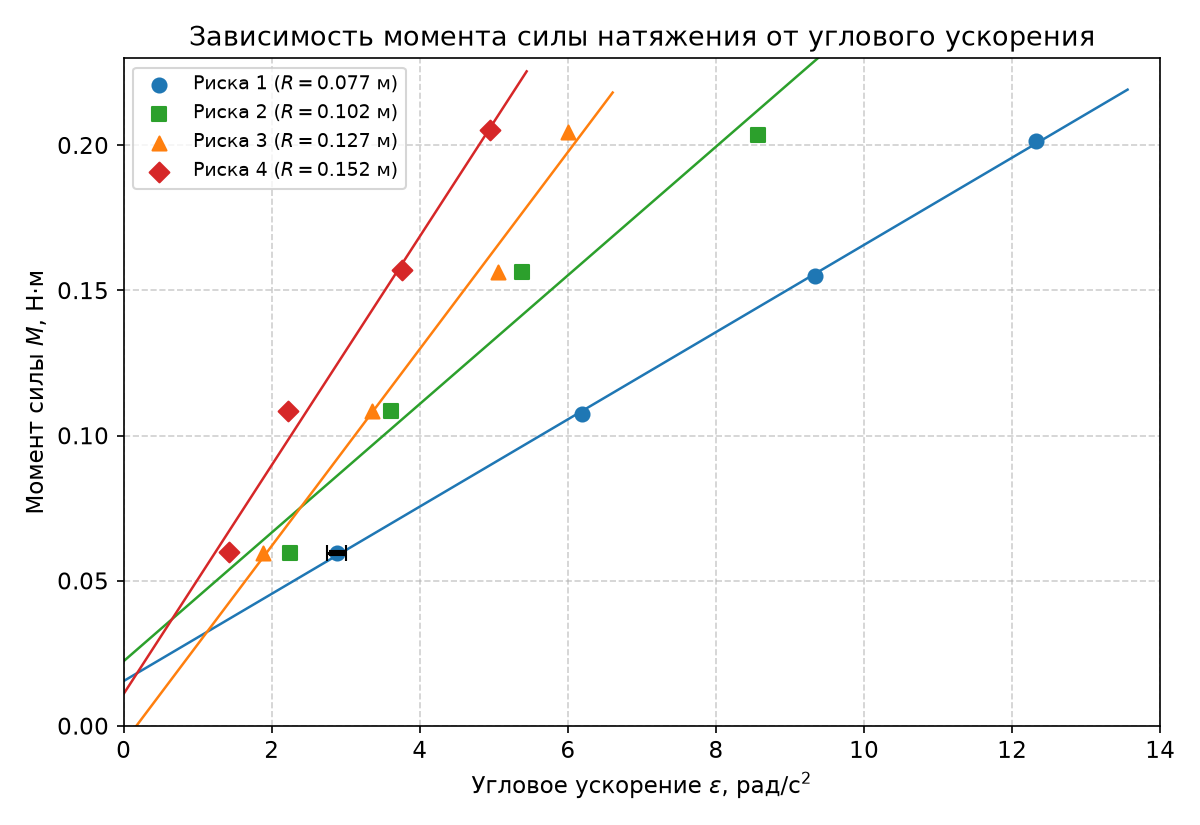
\includegraphics[width=0.85\textwidth]{assets/graph1.png}}
    \caption{Зависимость момента силы натяжения \(M\) от углового ускорения \(\varepsilon\) для различных положений грузов}
    \label{fig:graph1}
\end{figure}

\begin{figure}[H]
    \centering
    \fbox{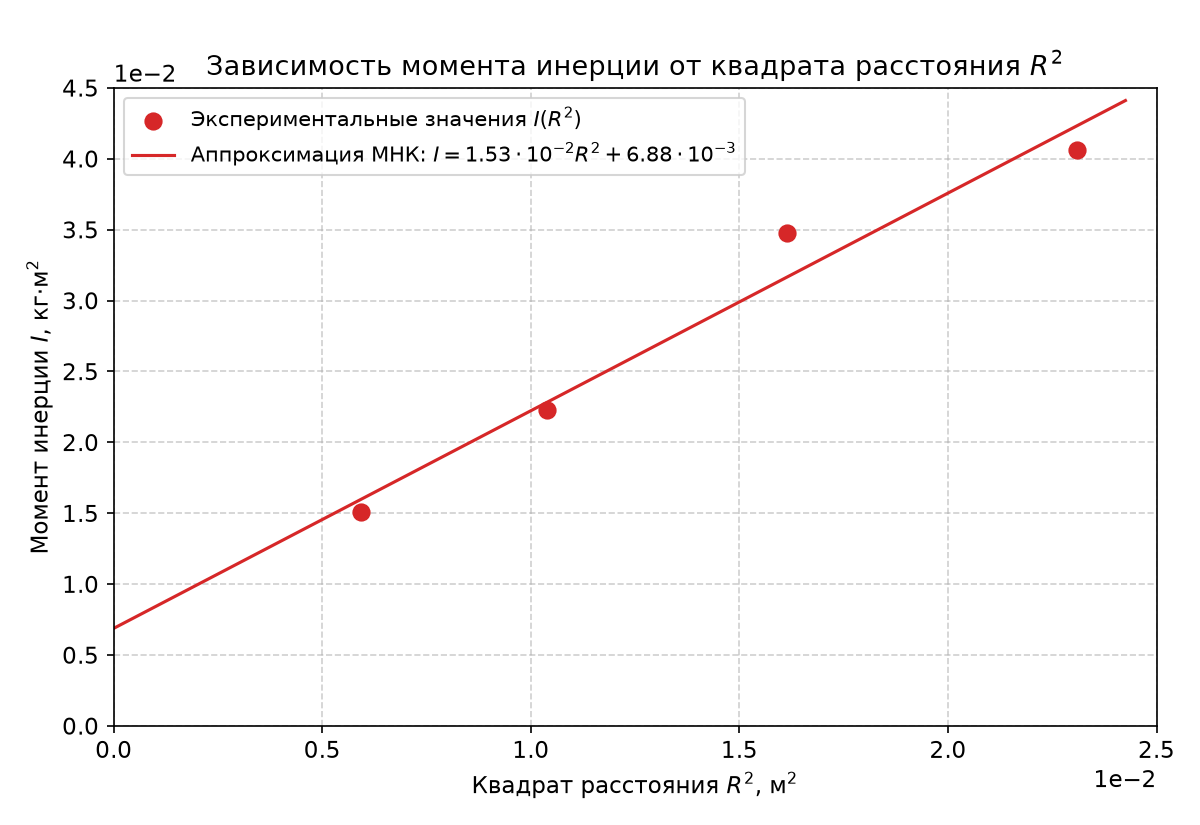
\includegraphics[width=0.85\textwidth]{assets/graph2.png}}
    \caption{Зависимость момента инерции \(I\) от квадрата расстояния \(R^2\) (теорема Штейнера)}
    \label{fig:graph2}
\end{figure}

\end{document}